% !TEX root = main.tex

\section{Задача №4. Доверительные интервалы}

\paragraph{Условие.} Среднее значение дальности до ориентира, полученного по результатам $n = 10$ независимых измерений, равно 3230 м. Считая, что ошибки измерения распределены по нормальному закону с нулевым математическим ожиданием, а среднее квадратичное отклонение ошибки составляет $\sigma=8$ м, найти 95\%ый доверительный интервал для дальности ориентира.
\paragraph{Решение.}
Пусть 
\begin{enumerate}
	\item $m$ -- теоритическое значение дальности до ориентира;
	\item $X$ -- случайная величина, принимающая значения, равные измеренной дальности до ориентира.  
\end{enumerate}

\[
X = m + (error)
\]

По условию
 \[
(error) \sim N(0, \sigma^2) 
\]

Тогда 
\[
X \sim N(0, \sigma^2), \sigma = 8
\]
\[
\Expect\left[m + (error)\right] = m + \Expect\left[error\right] = m
\]

Таким образом необходимо оценить $m$.
Используес статистику

\[
T(\vec{X}) = \frac{m - \bar{X}}{\sigma} \sqrt{n} \sim N(0, 1);
\]

\begin{figure}[h!]
	\begin{center}
		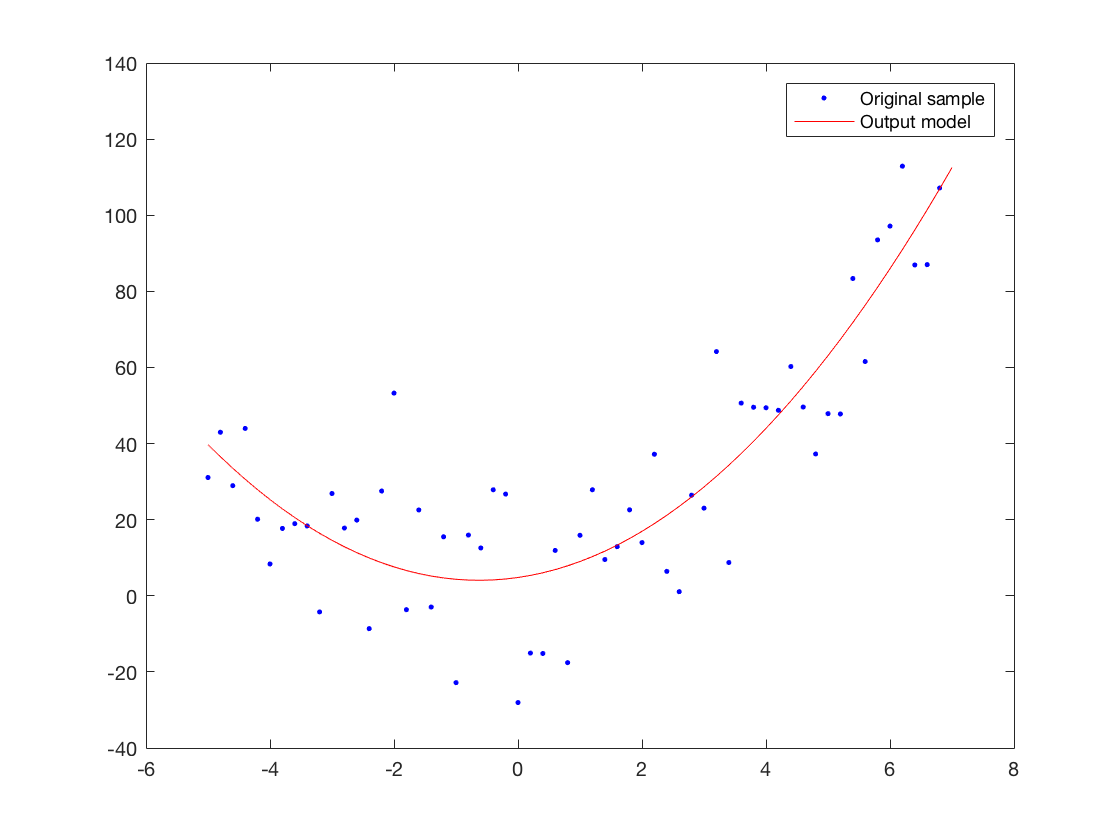
\includegraphics[width=300px]{1.png}
	\end{center}
\end{figure}

\[
\Prob \{-u_{0.975} < T < u_{0.975}\} = \gamma;
\]

\[
\Prob \{-u_{0.975} <   \frac{m - \bar{X}}{\sigma} \sqrt{n}  < u_{0.975} \} = \gamma;
\]

\[
\Prob \{ \bar{X} - \frac{\sigma u_{0.975}}{\sqrt{n}}  < m <  \bar{X} + \frac{\sigma u_{0.975}}{\sqrt{n}} \} = \gamma;
\]

Примем за $\underline{m}(\vec{X}) = \bar{X} - \frac{\sigma u_{0.975}}{\sqrt{n}} $ и $\bar{m}(\vec{X}) = \bar{X} +\frac{\sigma u_{0.975}}{\sqrt{n}}$

\[
u_{0.975} = 1.977
\]

\[
\frac{\sigma u_{0.975}}{\sqrt{n}} = \frac{8 * 1.977}{\sqrt{10}} = 5.001 \approx 5
\]

\[
\bar{X} = 3230
\]

Таким образом $\underline{m} = 3230 - 5 = 3225$ и $\bar{m} = 3230 + 5 = 3235$
\paragraph{Ответ.} $3225 < m < 3235$